\documentclass{urticle}
\begin{document}

\begin{center}
    {\bf \Large Саморепродукция и эффект Талбота}
\end{center}

\newpage

\section{Теоретическая часть}
\subsection{Саморепродукция}

    Если рассмотреть дифракцию на предмете, имеющем некую периодескую структуру, то можно будет пронаблюдать эффект саморепродукции: на некотором расстоянии от предмета вдоль распространения волны появится изображение той же переодической структуры. Физическая природа этого эффекта заключается в том, что при прохождении волны через периодечкую структуры комплексная амплитуда волны, идюущая после предмета будет тоже периодичной. В таком случае будет существовать плоскость, в которой волны, прищедшие от предмета, будут иметь задержку, крутную $2\pi$. И тогда в этой плоскости возникнет репродуцированное изображение. 

    Пусть на нашу периодечскую структуру падает монохроматическая волна:
    \begin{equation}
        E(r,t) = a_0 e^{-i(\omega t- \bf{kr} - \psi_0)}
    \end{equation}
    Согласно определению плоской волны, колебания просиходят синфазно во всех точках плосксоти: 
    \begin{equation}
        \textbf{kr} = xu - yv - z\sqrt{k^2-u^2-v^2} = const
    \end{equation}
    где $u$ и $v$ -- пространственные частоты, определямые напрвлением вектора $\bf{k}$. Тогда комплексная амплитуда такой волны записывается в виде:
    \begin{equation}
        f(x,y,z) = a_0 e^{i\psi_0}e^{i(xu+yv)}e^{iz\sqrt{k^2-u^2-v^2}} = f(x,y,0)e^{iz\sqrt{k^2-u^2-v^2}}
    \end{equation}
    Тогда поле в плоскости z = 0 однозначно определяет поле плоскости z = \textit{const}. 

    Пусть $t(x,y)$ - функция пропускания траспоранта. И пусть она явлется периодичсекой с периодом d. А тогда и волновой фронт, в плоскости z = 0 имеет тот же период. Значит такую функцию можно разложить в ряд фурье с кратными пространственными частотами $u_n = {2\pi n}/{d}$ и $v_m = {2\pi m}/{d}$:
    \begin{equation}
        f(x,y,0) = \sum_{n=-\infty}^{\infty} \sum_{m=-\infty}^{\infty} c_{nm} e^{i u_n x} e^{i v_m y} = \sum_{n=-\infty}^{\infty} \sum_{m=-\infty}^{\infty} c_{nm} e^{i\frac{2\pi}{d}nx} e^{i\frac{2\pi}{d}my}
    \end{equation}
    Тогда значение комплексной амплитуды в произволной плоскости z = \textit{const} имеет вид:
    \begin{equation}
        f(x,y,z) = \sum_{n=-\infty}^{\infty} \sum_{m=-\infty}^{\infty} c_{nm} e^{i\frac{2\pi}{d}nx} e^{i\frac{2\pi}{d}my} e^{iz\sqrt{k^2-u_n^2-v_m^2}}
    \end{equation}
    Получается каждая плоская волна в суперспозиции (4) при распространении от транспоранта до плоскости z = \textit{const} приобрела набег фаз: 
    \begin{center}
        $ \varphi_{nm} = \sqrt{k^2-u_n^2-v_m^2} \cdot z $
    \end{center}      
    Который с учетом фринелевского приблежения можно представить в виде:
    \begin{equation}
        \varphi_{nm} \approx kz - \frac{u_n^2 + v_m^2}{2k}z
    \end{equation}
    Тогда набег фаз между двумя любыми плоскими волнами (с индексами $n, m$ и $p, q$) равен:
    \begin{equation}
        \Delta \varphi_{nm} = (u_n^2 + v_m^2 - u_p^2 - v_q^2)\frac{z}{2k} = (n^2+m^2-p^2-q^2)\frac{\pi\lambda}{d^2}z
    \end{equation}
    Тогда если в какой-то плоскости эта разница фаз равна $2\pi$, то в результате интерференции волн воспроизведется картина, которая находится в плоскости z = 0 т.е. повторит эту периодическую структуру. И такие плоскости соотвествуют:
    \begin{equation}
        z_N = \frac{2d^2}{\lambda}N
    \end{equation}
    
\subsection{Число <<копий>>}

    \begin{wrapfigure}[13]{r}{0.5\linewidth} 
        \vspace{-5ex}
        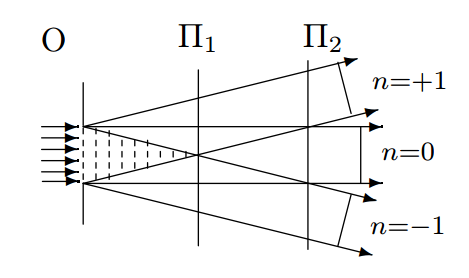
\includegraphics[width=\linewidth]{1.png}
        \caption{Зависимость освещенности в максимуме от высоты входной щели}
        \label{f1}
    \end{wrapfigure}

    В предшествующих выводах мы никак не учитывали, что периодическая структура имеет конечные размеры. Для конкретики, рассмотрим дифракционную решетку. За счет дифракционного уширения, картина после щели будет выглядить, если мы нарисуем три продифрагированных луча порядков n = \{-1, 0, 1\} (рис.~\ref{f1})

    Оценим максимальное число <<копий>> решетки длиной D. Три волны перестают перекрываться на расстоянии L между плоскостями O и П$_1$:
    \begin{equation}
        L = \frac{D}{2}\ctg\theta,
    \end{equation}
    где $\theta$-- угол дифракции, который определяется из условия $d\sin\theta = \lambda$. Тогда за счет параксиальности лучей получим:
    \begin{equation}
        L \approx \frac{D}{2\theta} \approx \frac{Dd}{2\lambda}
    \end{equation}
    И тогда на этом расстоянии число плосксотей саморепродукции состовляет
    \begin{equation}
        N \approx \frac{L}{z_1} \approx \frac{D}{4d}
    \end{equation}
\newpage
\subsection{Ковер Талбота}
    Рассмотрим в качестве периодической структуры дифракционную решетку с периодом d. А на экран падает плоская волна вдоль оси z:
    \begin{equation}
        E(x,z) = a_0 e^{ikz} e^{-i\omega t}
    \end{equation}        
    Тогда c учетом (12) выражение (5) представляется в виде:
    \begin{equation}
        f(x,z) = \sum_{n=-\infty}^{\infty} c_{n} e^{i u_n x}e^{iz\sqrt{k^2-u_n^2}} = e^{ikz} \sum_{n=-\infty}^{\infty} c_{n} e^{i( u_n x -\frac{u_n^2}{2k}z)} = e^{ikz} \sum_{n=-\infty}^{\infty} c_{n} e^{i \frac{2\pi}{d}n(x -\frac{\pi n}{kd}z)}
    \end{equation}
    Эффект саморепродукции конечно проявляется и в этом случае. Но больший интерес представляет картина интесивности на одном периоде (см. рис.~\ref{f2})
    \begin{figure}[h]
        \begin{center}
            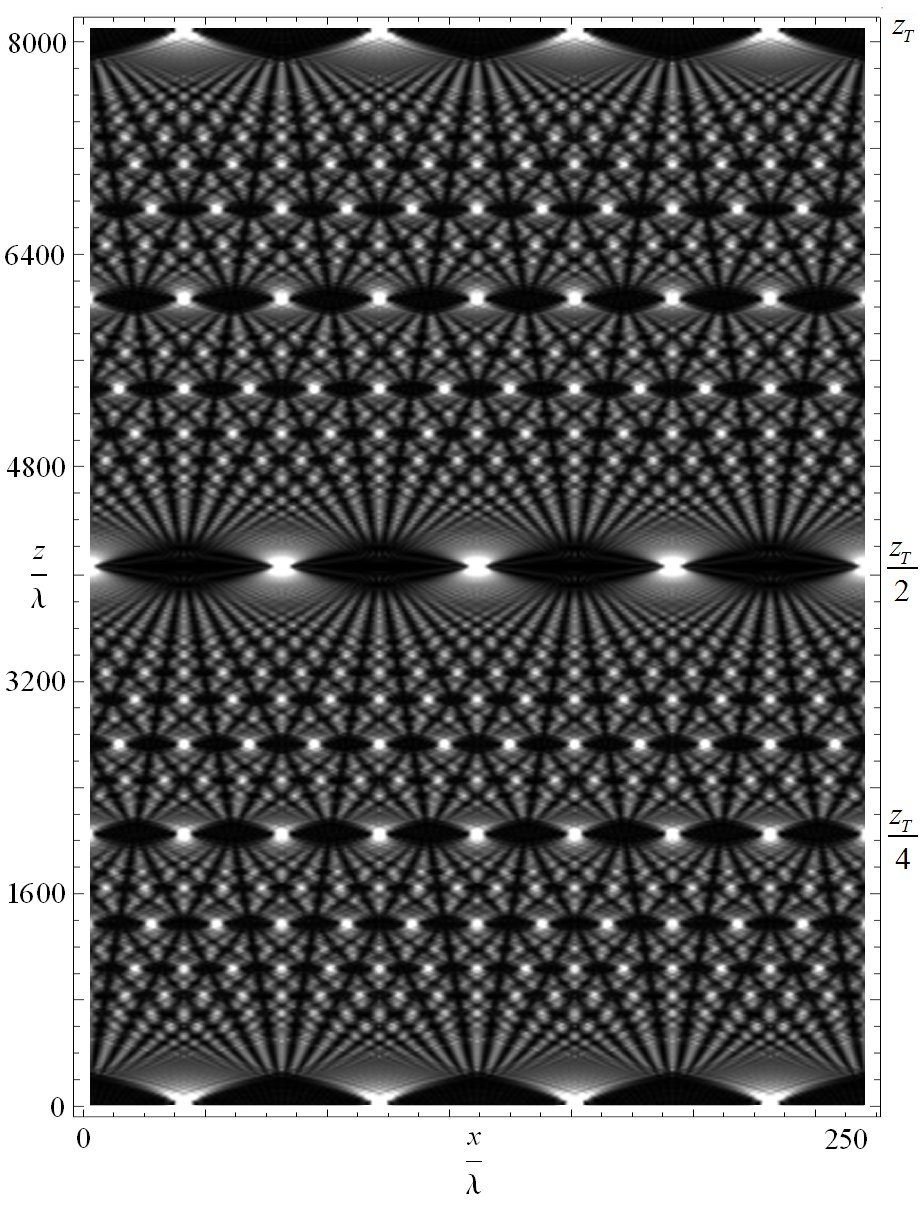
\includegraphics[scale=0.3]{2.png}
        \end{center}
        \caption{Ковер Талбота}
        \label{f2}
    \end{figure}
    
\newpage    
\section{Экспериментальная часть}
\subsection{Экспериментальная установка}

    В качестве хорошего приблежени плоской волны будет служить лазер. На рис.~\ref{f3} можно увидеть принципиальную схему установки. 
    \begin{figure}[h]
        \begin{center}
            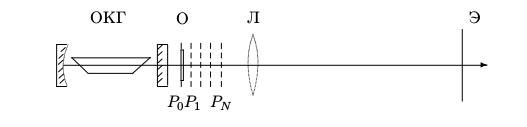
\includegraphics[scale=0.7]{3.png}
        \end{center}
        \caption{Схема установки: ОКГ -- гелий-неоновый лазер, О -- двумерная решетка, P$_N$ -- плоскости саморепродукции, Л -- короткофокусная линза, Э -- экран}
        \label{f3}
    \end{figure}
    
    С помощью линзы мы можем сфокусировать изображение находяющиеся в любой из плоскостей P$_N$ или между ними. В нашем случае вместо экрана будет выступать диафрагма фотоаппарата. И перемещая линзу с помощью микрометрического винта проделаем ряд снимков. После чего обработаем их на компьютере, для получения похожей картинки с рис.~\ref{f2}.
    
\section{Обработка результатов}


\end{document}
